\documentclass{article}
\usepackage[utf8]{inputenc}
\setlength\parindent{0pt}
\usepackage{nopageno}
\usepackage{amsmath}
\usepackage{amsfonts}
\usepackage{comment}

\title{A Better Confidence Interval for Proportions}
\author{}
\date{}

\usepackage{natbib}
\usepackage{graphicx}
\usepackage{amsmath}
\begin{document}

\maketitle 

\section*{The Problem with Small Samples}

The CLT guarantees that the sample proportion $\hat{p}$ is asymptotically normal, but the confidence interval is not guaranteed to be between $[0, 1]$, and is generally not efficient. This post demonstrates how the Delta Method can yield a much better confidence interval, and the calculation required to do so is very simple.

Under the Central Limit Theorem, $\hat{p} \sim \text{N}(0, \frac{p(1-p)}{n})$ as $n\rightarrow\infty$. We can use this to give a confidence interval for p: $$\widehat{\text{CI}(p)}=\hat{p} \pm q_\alpha\sqrt{\frac{p(1-p)}{n}}$$ where $\alpha$ is the false positive rate and $q_\alpha:=\int_{x=1-\alpha/2}^\infty \mathbb{P}(N(0, 1) = x)$. But for small $n$, this won't be exact because $p\in [0, 1]$, but $\widehat{\text{CI}(p)}$ could be outside $[0, 1]$. Generally, for small $n$, we don't have any guarantee that $100\cdot(1-\alpha)\%$ of the confidence intervals will contain $p$.

\section*{New Method}

For $x_1, ..., x_n \sim X$ with mean $\mu$ and variance $\sigma^2$, the CLT says: $$\sum x_i/n \sim N(\mu, \sigma^2/n)$$ as $n\rightarrow \infty$. Let's say we want to transform the sample average by appling a function $f$ to it. The CLT still applies! Specifically:

$$f(\sum (x_i)/n) \sim N(f(\mu,\sigma^2/n\cdot \left[f'(\mu)\right]^2)$$

This is called the Delta Method. So here's an idea for how to make a better confidence interval for the proportion: I'll tranform $\hat{p}$ to range between $(-\infty, \infty)$, find a confidence interval for that, then undo the transformation to the resulting lower and upper bounds so that they are also inside $[0, 1]$. Any function $f: [0, 1] \rightarrow (-\infty, \infty)$ will work, but I'll pick one similar to what we saw in class: $f(p)=\text{log}(\frac{p}{1-p})$.

\newpage
If you do the math, you'll see that $f'(p) = \frac{1}{p(1-p)}$, and $f^{-1}(z) = \frac{e^z}{1+e^z}$. So the Delta Method says the CLT on the transformed proportion is:

$$f(\hat{p}) \sim N\left(f(p),\ \frac{1}{p(1-p)n}\right)$$

and the transformed confidence interval is:

$$(\text{lower}, \text{upper}) = f(\hat{p}) \pm q_\alpha\sqrt{\frac{1}{\hat{p}(1-\hat{p})n}}$$

To put get back a new confidence interval for $\hat{p}$, I'll apply $f^{-1}$ to the confidence interval bounds. That is, my new confidence interval is:$$\left(\frac{e^\text{lower}}{1+e^\text{lower}},\ \frac{e^\text{upper}}{1+e^\text{upper}}\right)$$

\section*{Performance}

For a range of true proportions $p$ and sample sizes $n$, we would like a confidence interval to actually contain the true proportion $100\cdot(1-\alpha)\%$ of the time. No more, no less. The following plots show that the traditional use of the CLT is reliably off-- specifically, it under-covers the true proportion in small sample sizes. The new method is pretty much spot on. Yay!

\ \\
Finally, I'm adding the code I wrote to create these simulations and plots.

\section*{Plots}
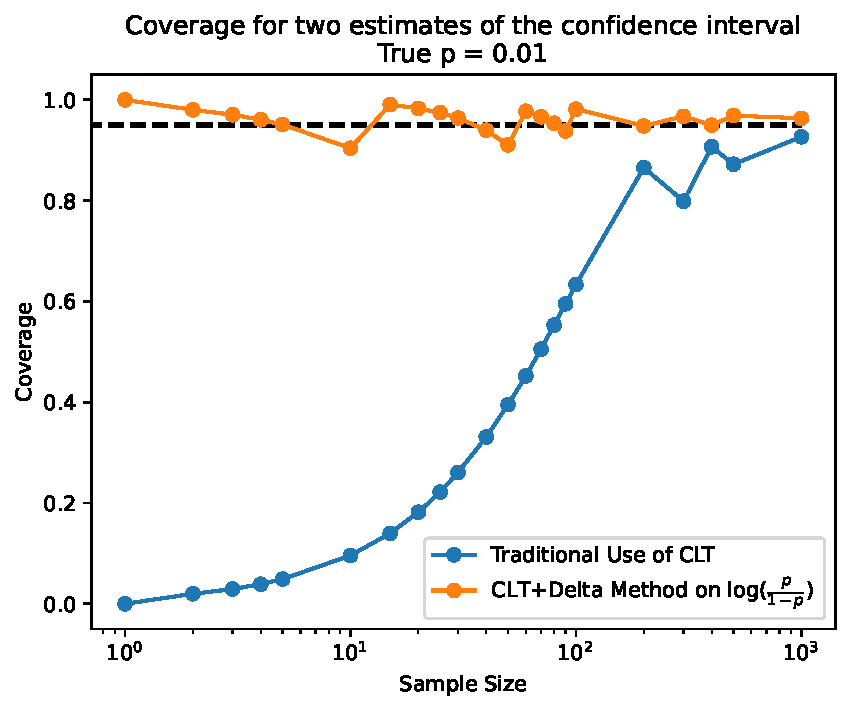
\includegraphics[width=13cm]{plot_0.pdf}
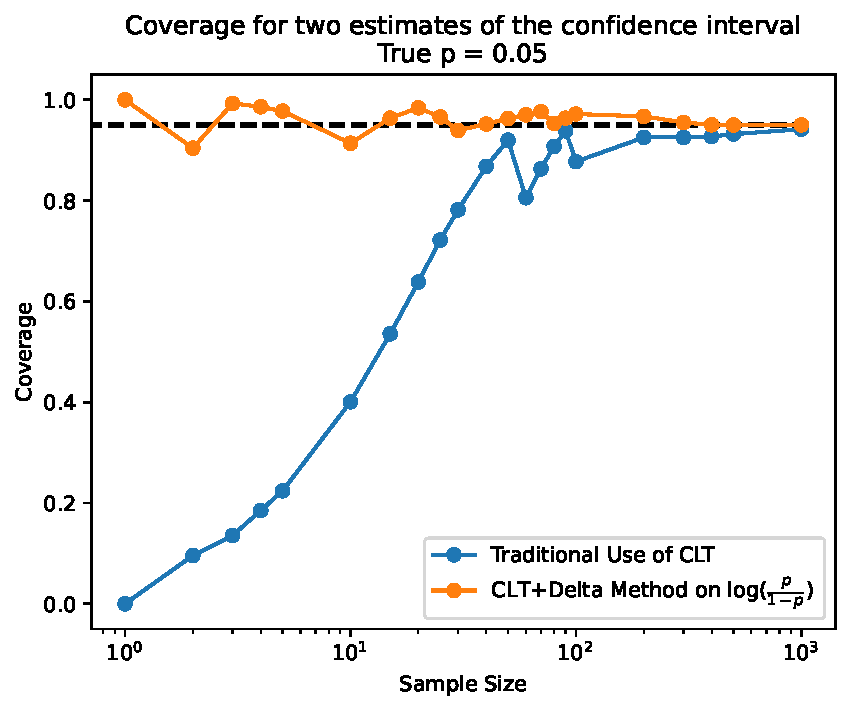
\includegraphics[width=13cm]{plot_1.pdf}
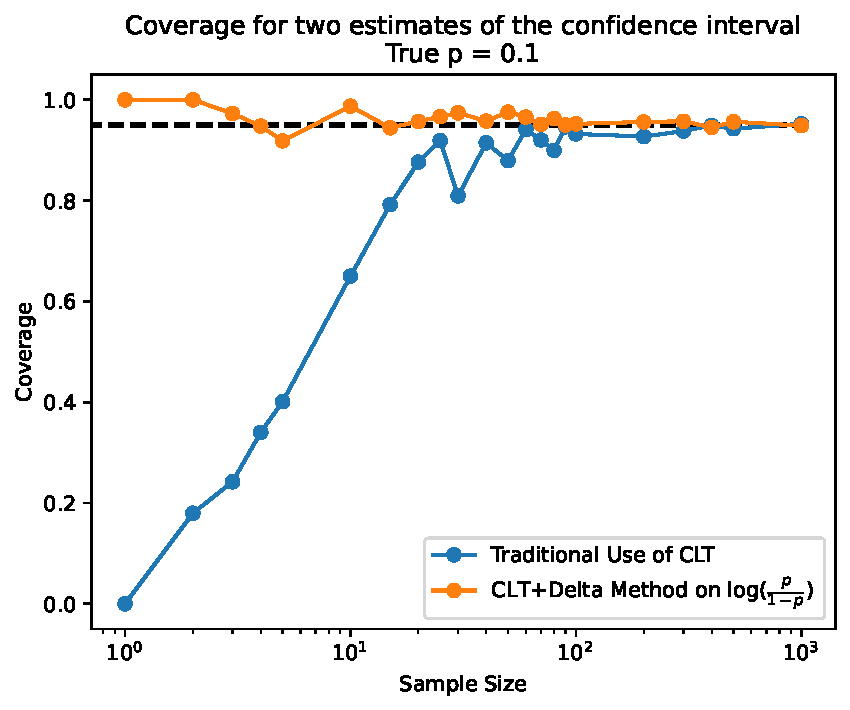
\includegraphics[width=13cm]{plot_2.pdf}
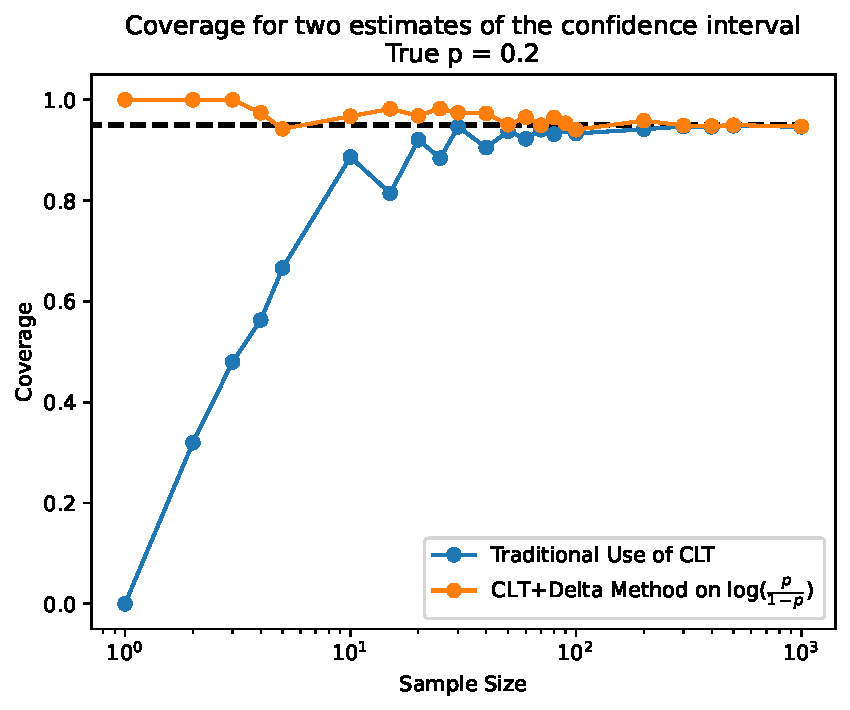
\includegraphics[width=13cm]{plot_3.pdf}
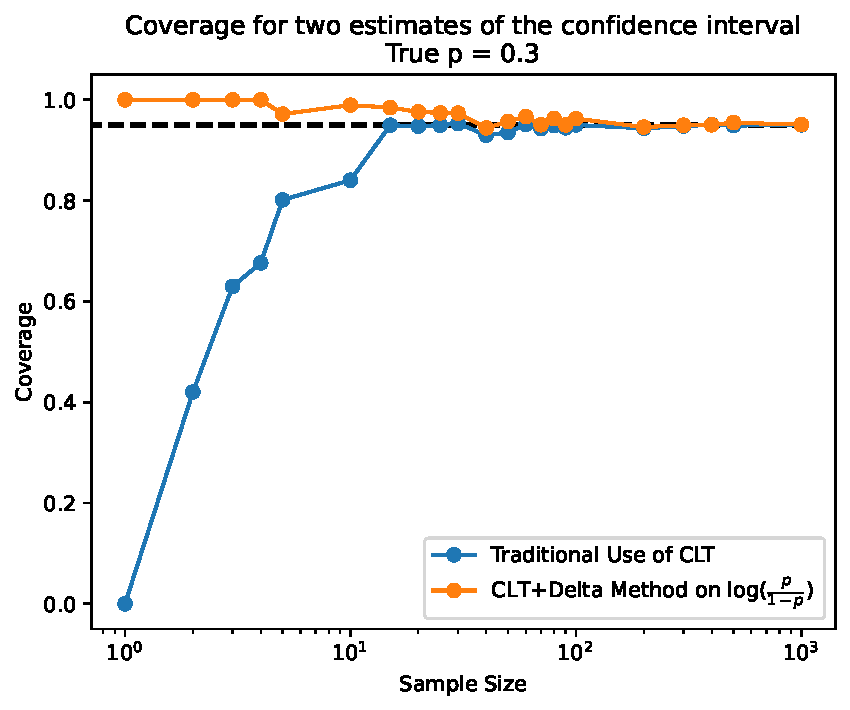
\includegraphics[width=13cm]{plot_4.pdf}

\newpage
\section*{Python Code}
\begin{verbatim}

import numpy as np
import scipy.stats as ss
import copy

def test(n, B, p, t=.01, alpha=.05):
    q = ss.norm(0, 1).ppf(1 - alpha/2)

    ### traditional method
    ph = ss.binom(n, p).rvs(B) / n
    old_coverage = np.logical_and(
        ph - q * np.sqrt(ph*(1-ph)/n) < p,
        ph + q * np.sqrt(ph*(1-ph)/n) > p
    )

    ### new method
    # nuisance: truncate so ph strictly between 0 and 1
    pht = copy.deepcopy(ph)
    pht[pht == 0] = t
    pht[pht == 1] = 1-t
    
    lower = np.log(pht/(1-pht)) - q  / np.sqrt((n * pht * (1-pht)))
    upper = np.log(pht/(1-pht)) + q  / np.sqrt((n * pht * (1-pht)))

    new_coverage = np.logical_and(
        np.exp(lower)/(1+np.exp(lower)) < p,
        np.exp(upper)/(1+np.exp(upper)) > p
    )
    return np.mean(old_coverage), np.mean(new_coverage)

\end{verbatim}
\newpage
\begin{verbatim}
ns = (1, 2, 3, 4, 5,
      10, 15, 20, 25, 30,
      40, 50, 60, 70, 80, 90, 100,
      200, 300, 400, 500, 1000)

ps = (.01, .05, .1, .2, .3)
tests = [np.array([test(n, B=1000000, p=p, t=.0001) for n in ns]) for p in ps]

for example_p_ix in range(5):
    plt.semilogx((0, max(ns)), (.95,)*2,
                 linewidth=2, linestyle="--", c="#000000")
    plt.plot(ns, tests[example_p_ix][:,0], "o-",
             label="Traditional Use of CLT")
    plt.plot(ns, tests[example_p_ix][:,1], "o-",
             label=r"CLT+Delta Method on log($\frac{p}{1-p}$)")
    plt.xlabel("Sample Size")
    plt.ylabel("Coverage")
    plt.title(f"Coverage for two estimates of the confidence interval\nTrue p
              = {ps[example_p_ix]}")
    plt.legend()
    plt.savefig(f"~/coverages/plot_{example_p_ix}.pdf",
                format="pdf", bbox_inches="tight")
    plt.close()
\end{verbatim}
\end{document}
